A continuación se presentan y comentan las gráficas más representativas obtenidas tanto para los algoritmos de multiplicación de matrices como para los de ordenamiento. Cada bloque inicia con una descripción general de qué mide cada figura y termina con las principales observaciones.

\subsubsection{Multiplicación de matrices}

Para este experimento consideramos matrices de tamaños \(n = 2^4,2^6,2^8,2^{10}\) en los tres tipos de estructura (densa, diagonal y dispersa), midiendo tiempo de ejecución y memoria consumida por los algoritmos Naive y Strassen.

\begin{figure}[H]
    \centering
    \begin{minipage}[t]{1\textwidth}
        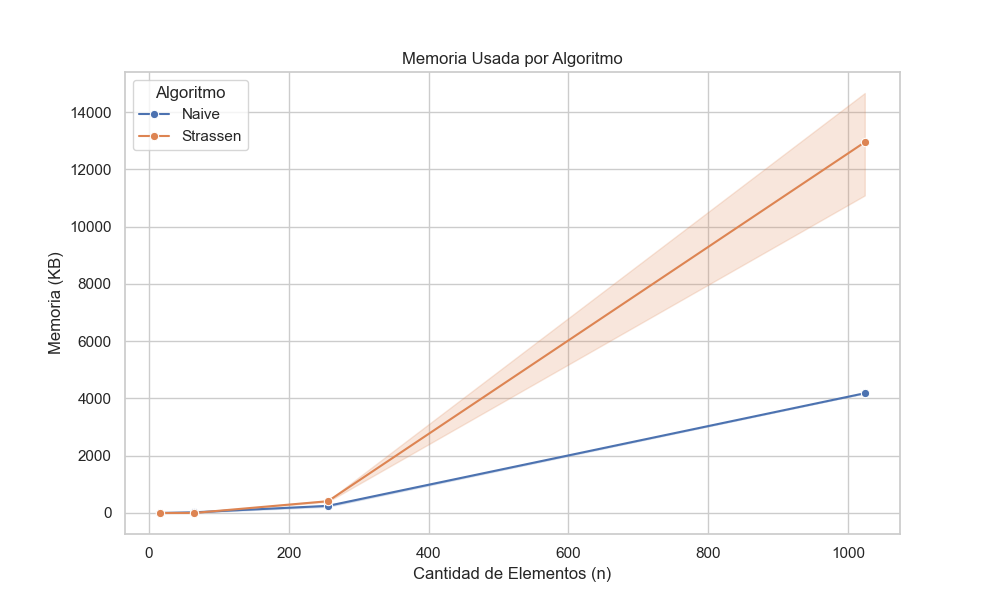
\includegraphics[width=\textwidth]{../code/matrix_multiplication/data/plots/memoria_vs_algoritmo.png}
     \end{minipage}%
    \caption{}
    \label{fig:scatterplot_3}
\end{figure}

\begin{figure}[H]
    \centering
    \begin{minipage}[t]{1\textwidth}
        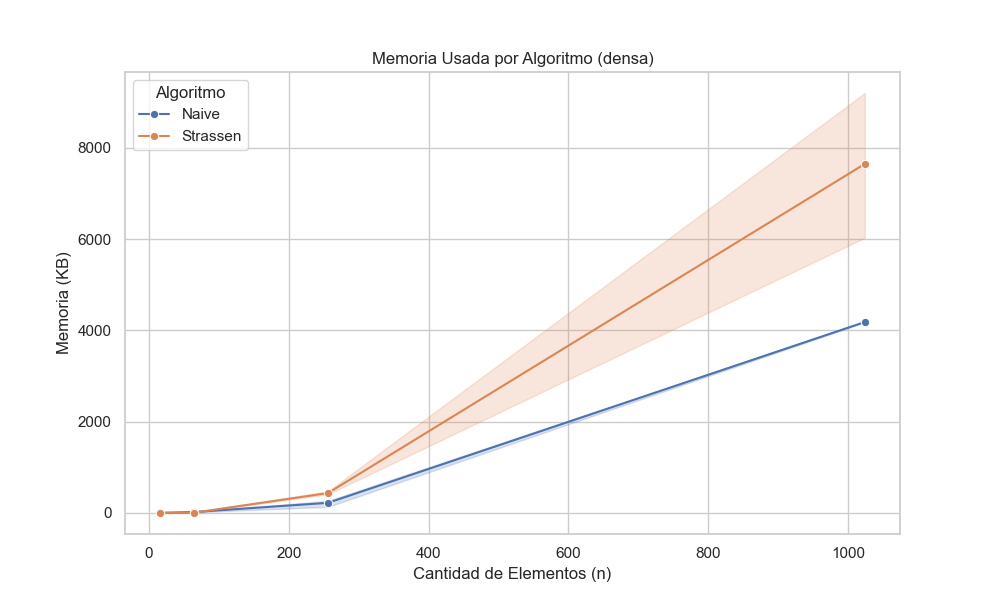
\includegraphics[width=\textwidth]{../code/matrix_multiplication/data/plots/memoria_vs_algoritmo_densa.png}
     \end{minipage}%
    \caption{}
    \label{fig:scatterplot_3}
\end{figure}

\begin{figure}[H]
    \centering
    \begin{minipage}[t]{1\textwidth}
        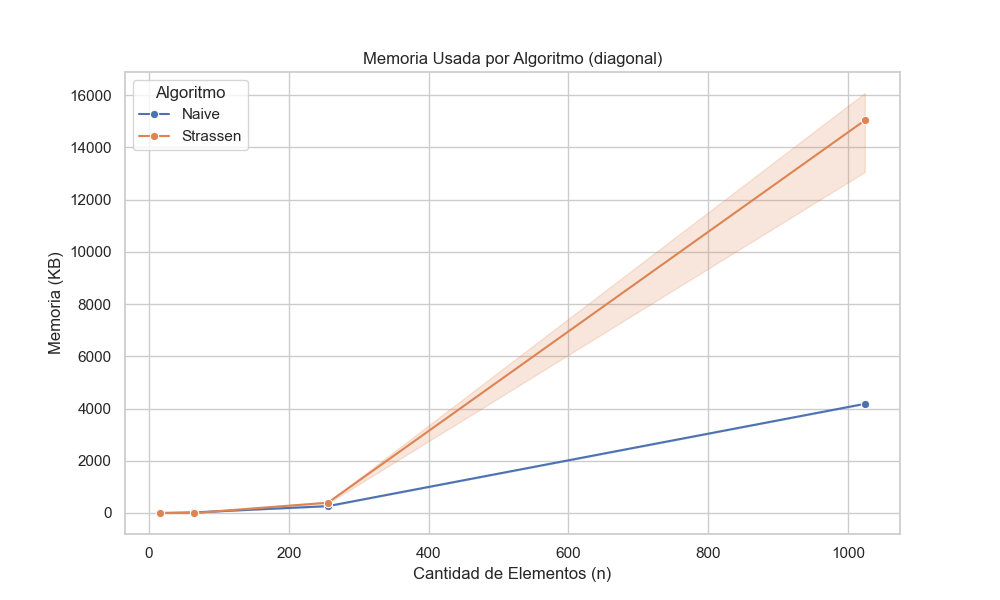
\includegraphics[width=\textwidth]{../code/matrix_multiplication/data/plots/memoria_vs_algoritmo_diagonal.png}
     \end{minipage}%
    \caption{}
    \label{fig:scatterplot_3}
\end{figure}

\begin{figure}[H]
    \centering
    \begin{minipage}[t]{1\textwidth}
        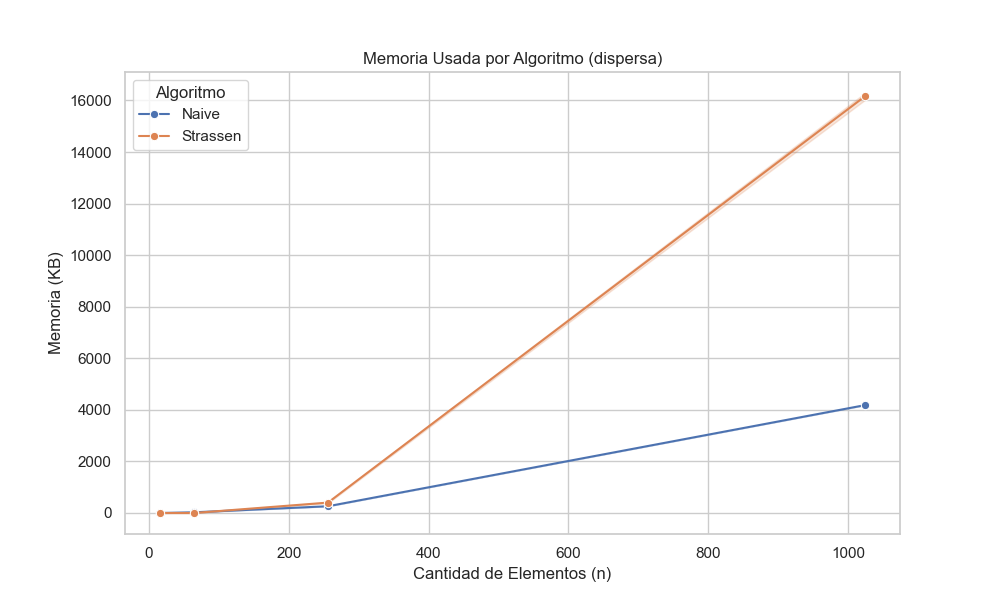
\includegraphics[width=\textwidth]{../code/matrix_multiplication/data/plots/memoria_vs_algoritmo_dispersa.png}
     \end{minipage}%
    \caption{}
    \label{fig:scatterplot_3}
\end{figure}

\begin{figure}[H]
    \centering
    \begin{minipage}[t]{1\textwidth}
        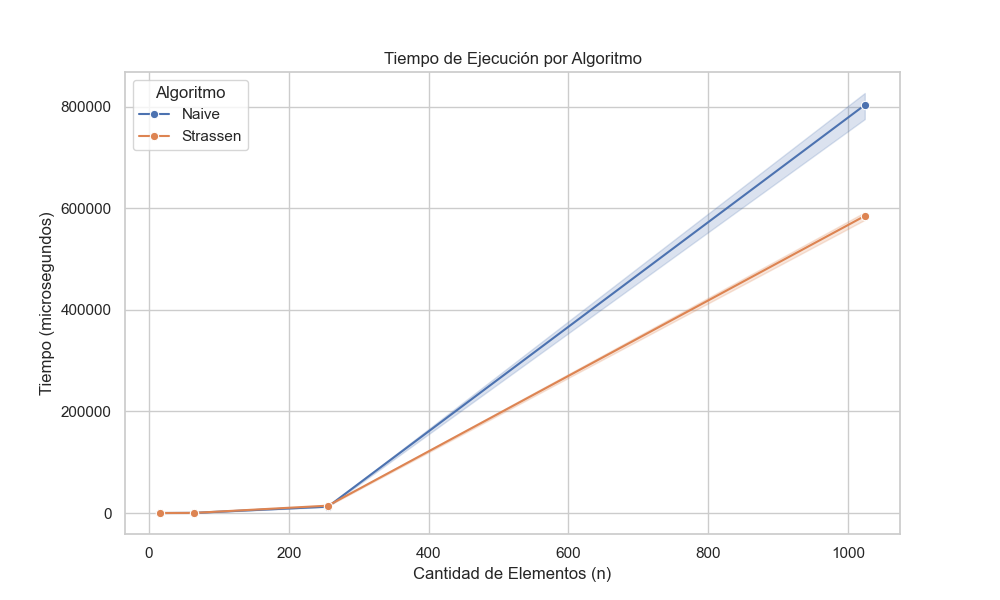
\includegraphics[width=\textwidth]{../code/matrix_multiplication/data/plots/tiempo_vs_algoritmo.png}
     \end{minipage}%
    \caption{}
    \label{fig:scatterplot_3}
\end{figure}

\begin{figure}[H]
    \centering
    \begin{minipage}[t]{1\textwidth}
        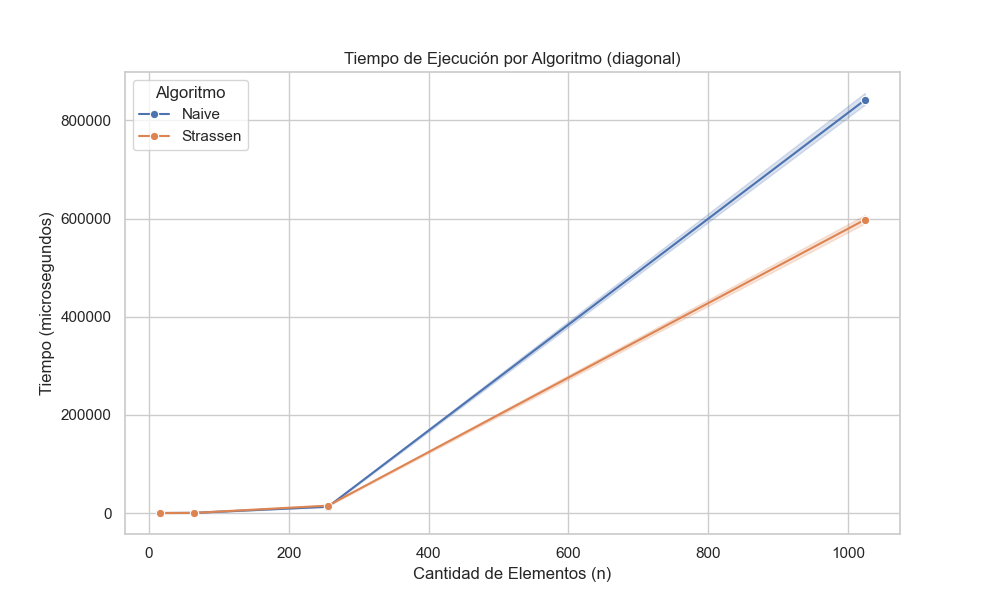
\includegraphics[width=\textwidth]{../code/matrix_multiplication/data/plots/tiempo_vs_algoritmo_diagonal.png}
     \end{minipage}%
    \caption{}
    \label{fig:scatterplot_3}
\end{figure}

\begin{figure}[H]
    \centering
    \begin{minipage}[t]{1\textwidth}
        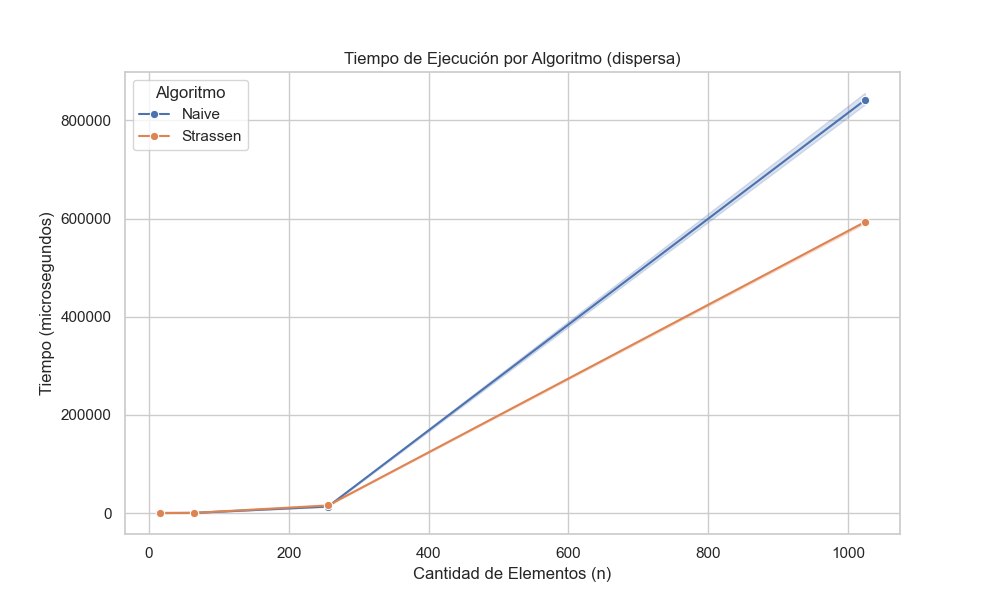
\includegraphics[width=\textwidth]{../code/matrix_multiplication/data/plots/tiempo_vs_algoritmo_dispersa.png}
     \end{minipage}%
    \caption{}
    \label{fig:scatterplot_3}
\end{figure}


\begin{itemize}
  \item \textbf{Memoria utilizada.}  
    \begin{itemize}
      \item El algoritmo Naive crece aproximadamente como \(O(n^2)\), reservando solo el espacio necesario para el producto final y unas pocas variables auxiliares.
      \item Strassen consume más memoria a medida que aumenta \(n\); esto se debe a las matrices temporales que crea en cada recursión, con un crecimiento cercano a \(O(n^{\log_2 7})\).  
    \end{itemize}

  \item \textbf{Tiempo de ejecución.}  
    \begin{itemize}
      \item El método Naive muestra un comportamiento cúbico \(O(n^3)\), con un aumento de tiempo muy acusado al duplicar la dimensión de la matriz.  
      \item Strassen reduce el tiempo efectivo, correspondiendo a su complejidad \(O(n^{2.807})\). La mejora es más evidente en tamaños grandes (\(n=2^8,2^{10}\)).  
      \item En matrices dispersas, ambos algoritmos tardan menos, pero la ventaja de Strassen permanece, aunque el overhead de recursión amortiza menos la ganancia para dimensiones pequeñas.  
    \end{itemize}
\end{itemize}

\begin{figure}[H]
    \centering
    \begin{minipage}[t]{1\textwidth}
        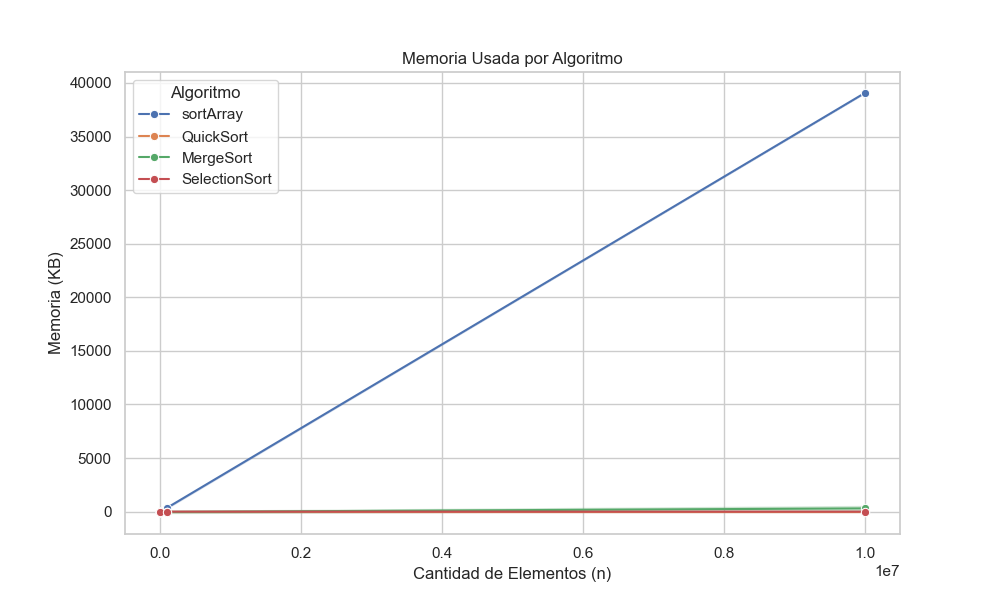
\includegraphics[width=\textwidth]{../code/sorting/data/plots/memoria_vs_algoritmo.png}
     \end{minipage}%
    \caption{}
    \label{fig:scatterplot_3}
\end{figure}

\begin{figure}[H]
    \centering
    \begin{minipage}[t]{1\textwidth}
        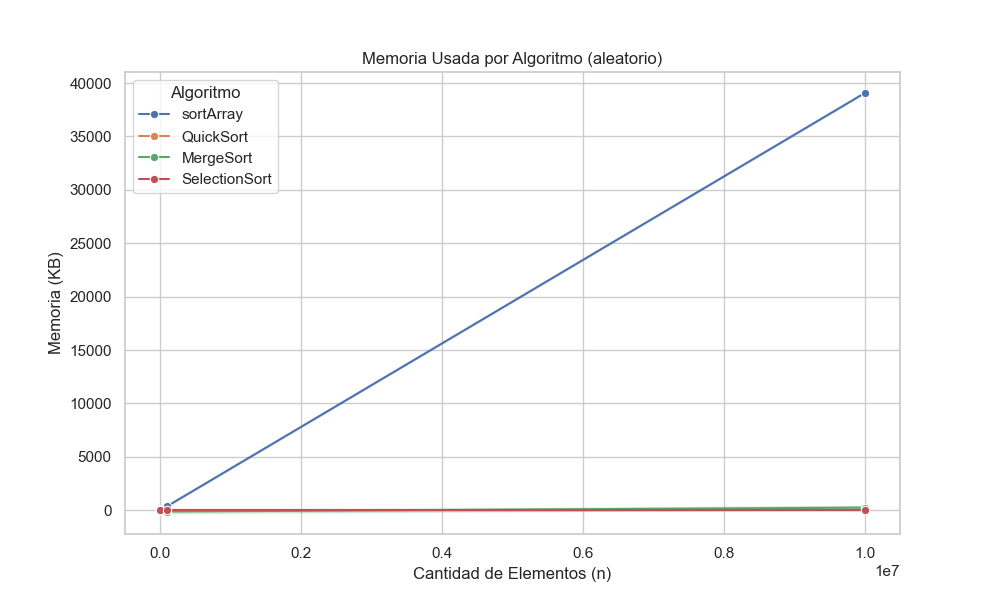
\includegraphics[width=\textwidth]{../code/sorting/data/plots/memoria_vs_algoritmo_aleatorio.png}
     \end{minipage}%
    \caption{}
    \label{fig:scatterplot_3}
\end{figure}

\begin{figure}[H]
    \centering
    \begin{minipage}[t]{1\textwidth}
        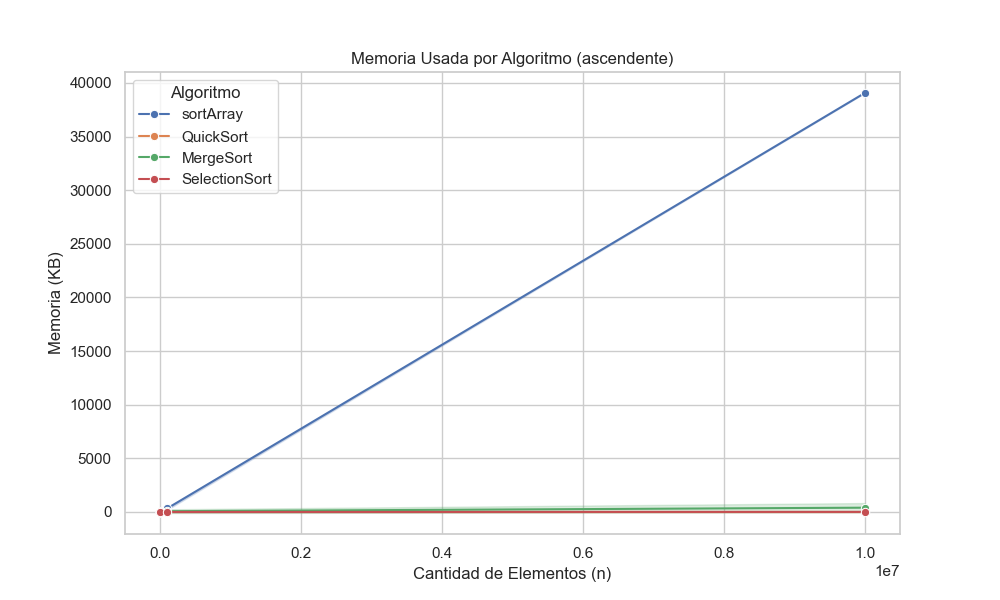
\includegraphics[width=\textwidth]{../code/sorting/data/plots/memoria_vs_algoritmo_ascendente.png}
     \end{minipage}%
    \caption{}
    \label{fig:scatterplot_3}
\end{figure}

\begin{figure}[H]
    \centering
    \begin{minipage}[t]{1\textwidth}
        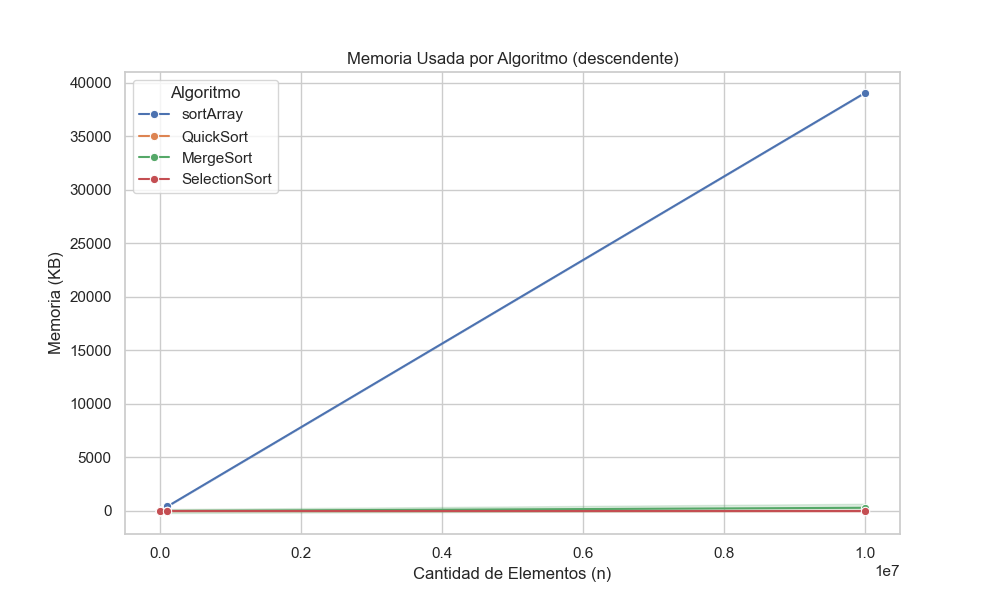
\includegraphics[width=\textwidth]{../code/sorting/data/plots/memoria_vs_algoritmo_descendente.png}
     \end{minipage}%
    \caption{}
    \label{fig:scatterplot_3}
\end{figure}

\begin{figure}[H]
    \centering
    \begin{minipage}[t]{1\textwidth}
        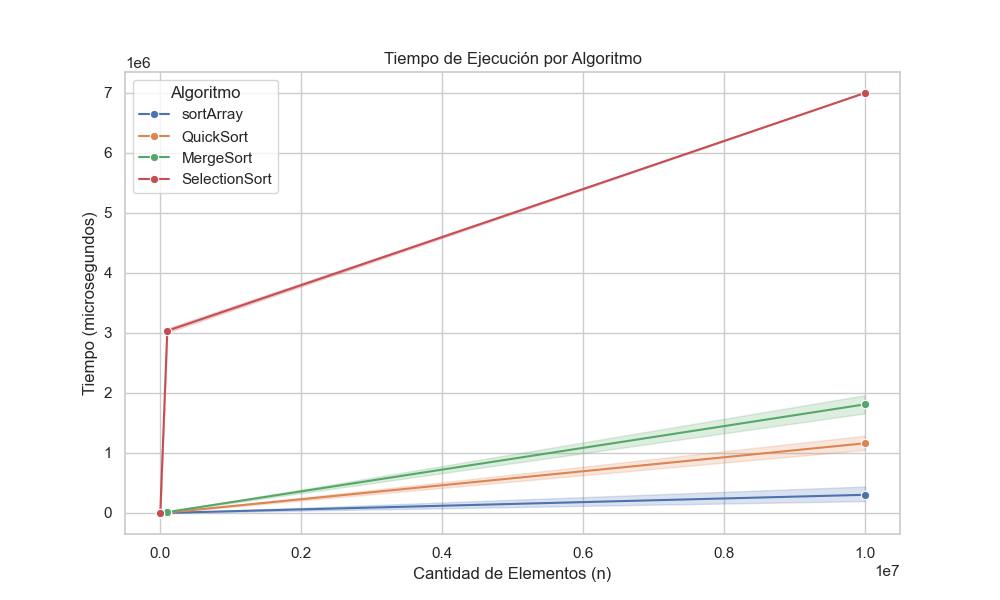
\includegraphics[width=\textwidth]{../code/sorting/data/plots/tiempo_vs_algoritmo.png}
     \end{minipage}%
    \caption{}
    \label{fig:scatterplot_3}
\end{figure}

\begin{figure}[H]
    \centering
    \begin{minipage}[t]{1\textwidth}
        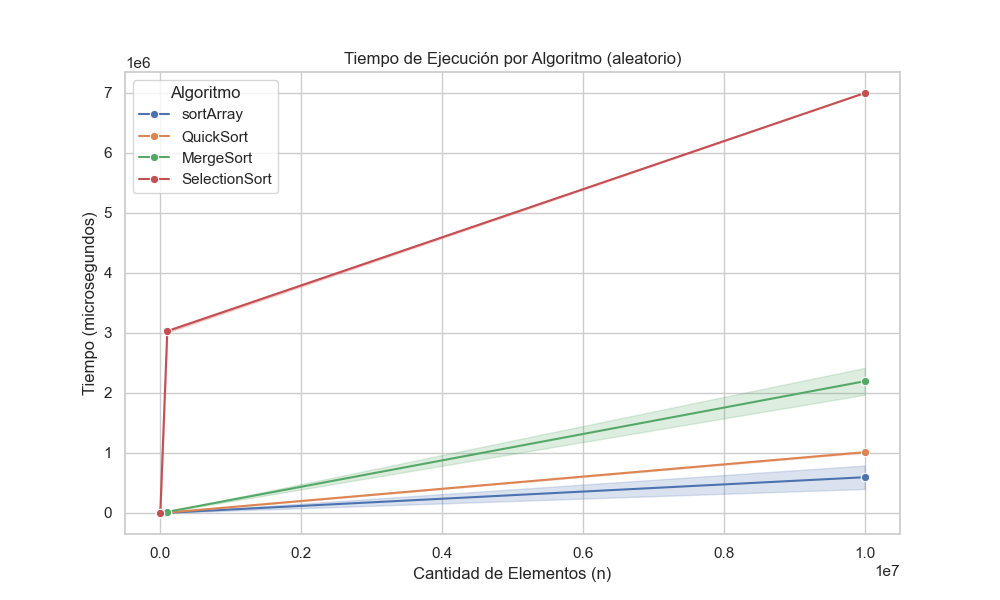
\includegraphics[width=\textwidth]{../code/sorting/data/plots/tiempo_vs_algoritmo_aleatorio.png}
     \end{minipage}%
    \caption{}
    \label{fig:scatterplot_3}
\end{figure}

\begin{figure}[H]
    \centering
    \begin{minipage}[t]{1\textwidth}
        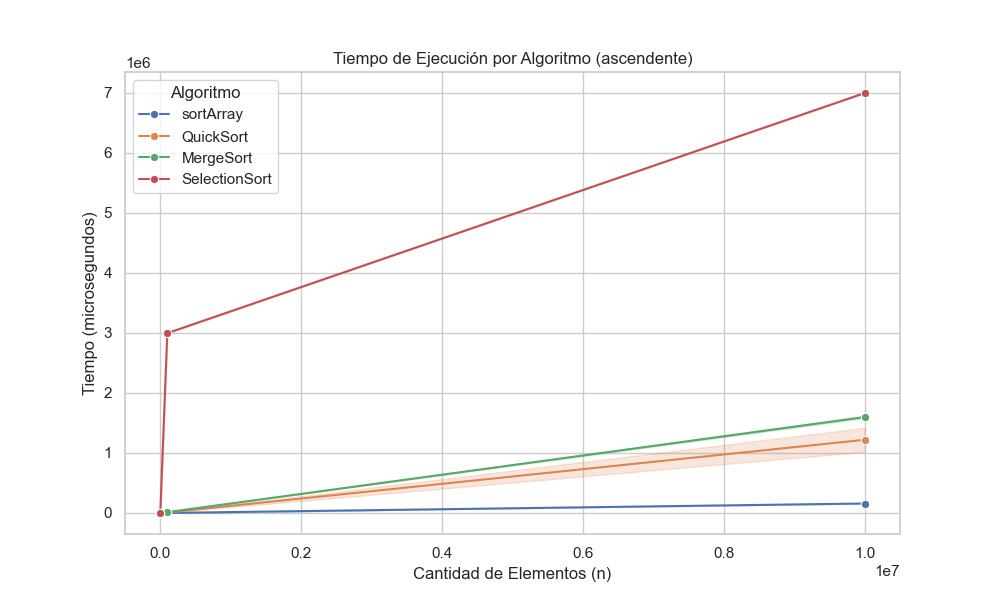
\includegraphics[width=\textwidth]{../code/sorting/data/plots/tiempo_vs_algoritmo_ascendente.png}
     \end{minipage}%
    \caption{}
    \label{fig:scatterplot_3}
\end{figure}

\begin{figure}[H]
    \centering
    \begin{minipage}[t]{1\textwidth}
        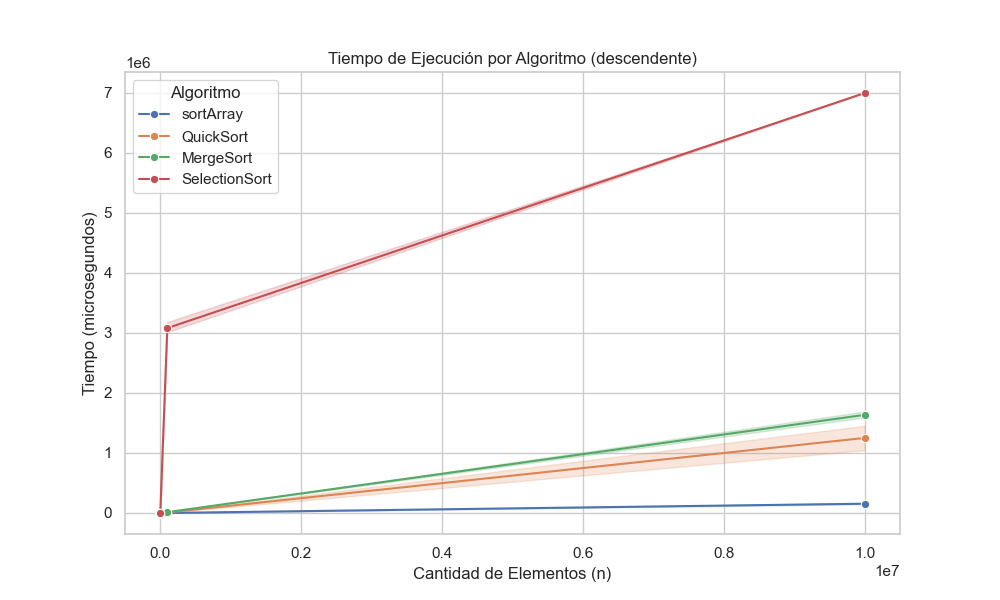
\includegraphics[width=\textwidth]{../code/sorting/data/plots/tiempo_vs_algoritmo_descendente.png}
     \end{minipage}%
    \caption{}
    \label{fig:scatterplot_3}
\end{figure}

\subsubsection{Ordenamiento}

Probamos cuatro algoritmos de ordenamiento sobre vectores de \(n=10^5,10^6,10^7\) elementos, en tres tipos de entrada (aleatoria, ascendente y descendente). Medimos tiempo de ejecución y memoria ocupada.

\begin{itemize}
  \item \textbf{Memoria utilizada.}  
    \begin{itemize}
      \item \texttt{sortArray} (\texttt{std::sort}) aloca internamente un buffer proporcional a \(n\), por lo que su consumo escala linealmente y es el mayor de los cuatro.  
      \item \texttt{MergeSort} también requiere \(O(n)\) espacio adicional para sus fusiones, aunque con menor constante que \texttt{std::sort}.  
      \item \texttt{QuickSort} utiliza espacio de pila \(O(\log n)\), prácticamente constante en comparación.  
      \item \texttt{SelectionSort} sólo emplea variables escalares, manteniéndose casi en \(O(1)\).  
    \end{itemize}
 
  
  \item \textbf{Tiempo de ejecución.}  
    \begin{itemize}
      \item \texttt{SelectionSort} evidencia su \(O(n^2)\): con \(n=10^7\) alcanza tiempos del orden de \(10^6\) ms, muy superior al resto.  
      \item \texttt{MergeSort} y \texttt{QuickSort}, ambos \(O(n\log n)\), crecen de forma similar; \texttt{QuickSort} es ligeramente más rápido en entradas aleatorias.  
      \item \texttt{std::sort} combina introsort y heapsort, mostrando el mejor desempeño en todos los casos, especialmente en entradas ya ordenadas (donde QuickSort puro puede degradarse).  
      \item La variación entre aleatorio, ascendente y descendente es mínima para Merge y \texttt{std::sort}, mientras que QuickSort sufre un pequeño pico en orden descendente si no se usa pivote aleatorio.  
    \end{itemize}
\end{itemize}

Para le generación de gráficos, se utilizó los scripts "plotgenerator.py" de ambos tipos de algoritmos, que fueron creados mediante los resultados obtenidos en la carpeta de "measurements" con el archivo "mediciones.csv".



